% Website with documentations on how to do trees
% https://latexdraw.com/draw-trees-in-tikz/
\section{Exercise A} 
\subsection{a)}

\begin{center}
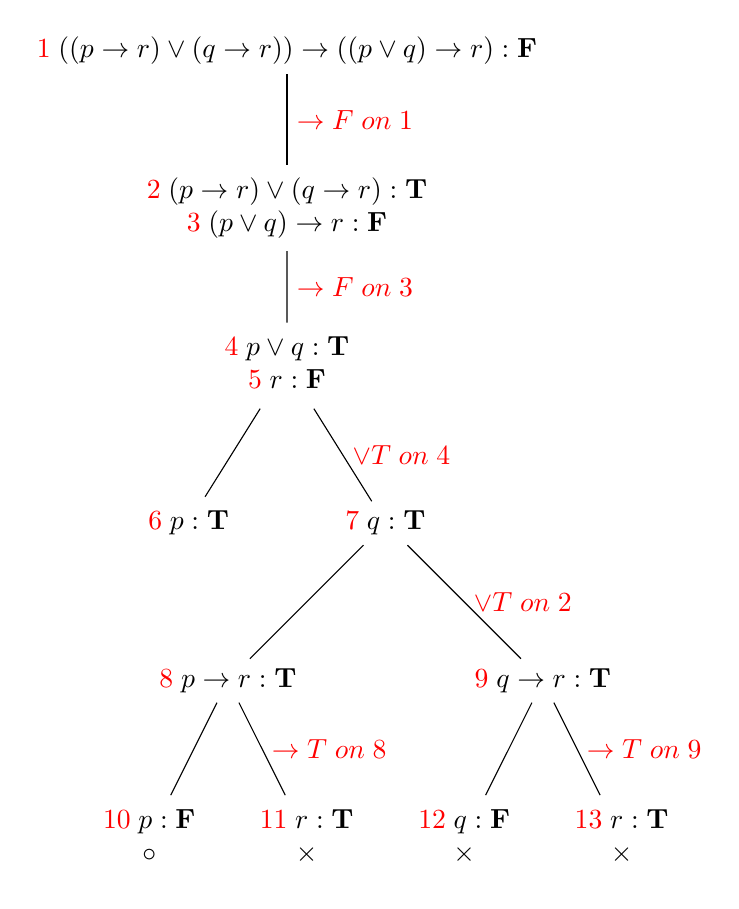
\begin{tikzpicture}

\node {$ \textcolor{red}{1}\; ((p \to r)\lor(q \to r))\to((p \lor q)\to r):\textbf{F} $} [sibling distance = 2.5cm] [level distance=20mm] 
        child {node {$ \begin{array}{c} \textcolor{red}{2}\; (p \to r)\lor(q \to r):\textbf{T} \\ \textcolor{red}{3}\; (p \lor q)\to r:\textbf{F} \end{array} $}  
            child {node {$ \begin{array}{c} \textcolor{red}{4}\; p \lor q:\textbf{T} \\ \textcolor{red}{5}\; r:\textbf{F} \end{array} $} 
                child {node {$ \begin{array}{c} \textcolor{red}{6}\; p:\textbf{T} \\ \end{array} $}}
                child {node {$ \textcolor{red}{7}\; q:\textbf{T} $} [sibling distance = 4cm]
                    child {node {$ \textcolor{red}{8}\; p \to r:\textbf{T} $} [sibling distance = 2cm]
                        child {node {$ \begin{array}{c} \textcolor{red}{10}\; p:\textbf{F} \\ \circ \end{array} $}}
                        child {node {$ \begin{array}{c} \textcolor{red}{11}\; r:\textbf{T} \\ \times \end{array} $}
                        edge from parent node [right, red] {$\to T\;on\; 8$}}} 
                    child {node {$ \textcolor{red}{9}\; q \to r:\textbf{T} $} [sibling distance = 2cm]
                        child {node {$ \begin{array}{c} \textcolor{red}{12}\; q:\textbf{F} \\ \times \end{array} $}}
                        child {node {$ \begin{array}{c} \textcolor{red}{13}\; r:\textbf{T} \\ \times \end{array} $ }
                        edge from parent node [right, red] {$\to T\;on\; 9$}}
                        edge from parent node [right, red] {$\lor T\;on\; 2$}}
                        edge from parent node [right, red] {$\lor T\;on\; 4$}}
                        edge from parent node [right, red] {$\to F\;on\; 3$}} 
                        edge from parent node [right, red] {$\to F\;on\; 1$}};

\end{tikzpicture}
\end{center}


The truth assignment that makes the formula false is:
\begin{itemize}
\item
p:\;\textbf{F}
\item
q:\;\textbf{T}
\item
r:\;\textbf{F}
\end{itemize}


\subsection{b)}

\begin{center}
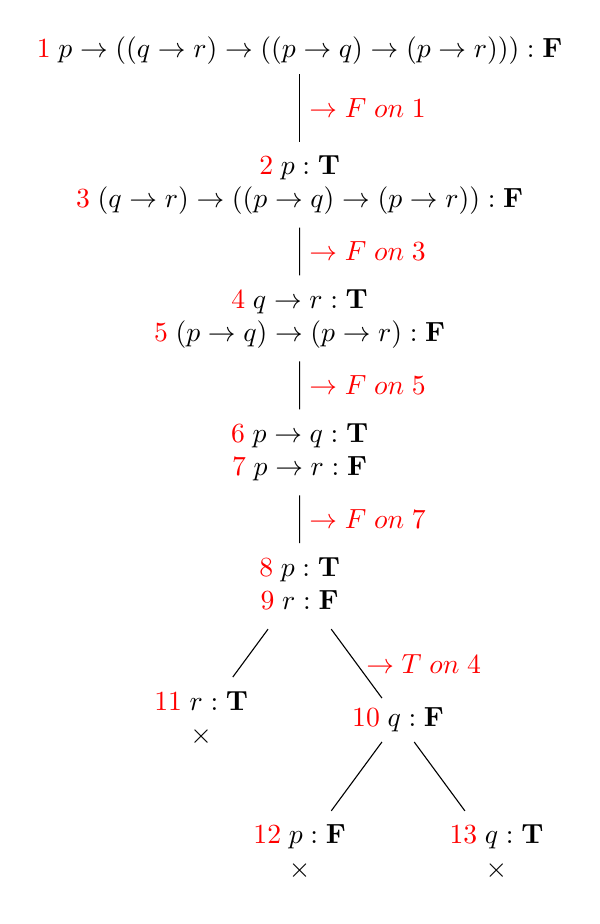
\begin{tikzpicture}

\node {$ \textcolor{red}{1}\; p \to ((q \to r)\to((p \to q)\to(p \to r))):\textbf{F} $} [sibling distance = 2.5cm] [level distance=17mm] 
        child {node {$ \begin{array}{c} \textcolor{red}{2}\; p:\textbf{T} \\ \textcolor{red}{3}\; (q \to r)\to((p \to q)\to(p \to r)):\textbf{F} \end{array} $} 
            child {node {$ \begin{array}{c} \textcolor{red}{4}\; q \to r:\textbf{T} \\ \textcolor{red}{5}\; (p \to q)\to(p \to r):\textbf{F} \end{array} $}
                child {node {$ \begin{array}{c} \textcolor{red}{6}\; p \to q:\textbf{T} \\ \textcolor{red}{7}\; p \to r:\textbf{F} \end{array} $}
                    child {node {$ \begin{array}{c} \textcolor{red}{8}\; p:\textbf{T} \\ \textcolor{red}{9}\; r:\textbf{F} \end{array} $}
                        child {node {$ \begin{array}{c} \textcolor{red}{11}\; r:\textbf{T} \\ \times \end{array} $}}
                        child {node {$ \textcolor{red}{10}\; q:\textbf{F} $}
                            child {node {$ \begin{array}{c} \textcolor{red}{12}\; p:\textbf{F} \\ \times \end{array} $}}
                            child {node {$ \begin{array}{c} \textcolor{red}{13}\; q:\textbf{T} \\ \times \end{array} $}}
                        edge from parent node [right, red] {$\to T\;on\; 4$}}
                        edge from parent node [right, red] {$\to F\;on\; 7$}}
                        edge from parent node [right, red] {$\to F\;on\; 5$}}
                        edge from parent node [right, red] {$\to F\;on\; 3$}} 
                        edge from parent node [right, red] {$\to F\;on\; 1$}};

\end{tikzpicture}
\end{center}

There is no truth assignment that makes the formula false, thus it is \underline{valid}.

